\documentclass{article}

\usepackage{soul}
\usepackage[margin=1in]{geometry}

\usepackage{listings}
\usepackage{color}

\usepackage{graphicx}
\graphicspath{ {./images/} }

\definecolor{dkgreen}{rgb}{0,0.6,0}
\definecolor{gray}{rgb}{0.5,0.5,0.5}
\definecolor{mauve}{rgb}{0.58,0,0.82}

\lstset{frame=tb,
  language=[Sharp]C,
  aboveskip=3mm,
  belowskip=3mm,
  showstringspaces=false,
  columns=flexible,
  basicstyle={\small\ttfamily},
  numbers=none,
  numberstyle=\tiny\color{gray},
  keywordstyle=\color{blue},
  commentstyle=\color{dkgreen},
  stringstyle=\color{mauve},
  breaklines=true,
  breakatwhitespace=true,
  tabsize=3
}

\date{\vspace{-7ex}}

\title{Haladó algoritmusok beadandó dokumentáció}
\author{Maár Kristóf - ISGK7K}

\begin{document}
\maketitle
\noindent

\section{Függvényközelítés megoldása genetikus algoritmussal}
\subsection{Bemenő paraméterek}

\begin{lstlisting}
  public class GASettings
  {
        public int NumberOfPopulation;
        public int NumberOfParents;
        public int ElitismNumber;
        public double FitnessToReach;
        public int MutationPercent;
        public string InputFilePath;
  }
\end{lstlisting}

\subsection{Forráskód}
  \begin{lstlisting}
    public class FA_With_GA
    {
        private static Random random = new Random();
        private GASettings settings;
        private FunctionApproximation functionApproximation;
        private Chromosome best;

        public FA_With_GA(GASettings settings)
        {
            this.settings = settings;
            functionApproximation = new FunctionApproximation(settings.InputFilePath);
        }

        public void SolveProblem()
        {
            List<Chromosome> population = InitializePopulation();
            best = GetBestChromosome(population);
            while (best.CalculateFitness(functionApproximation) > settings.FitnessToReach) // StopCondition
            {
                List<Chromosome> newPopulation = Elitism(population);

                while (newPopulation.Count != population.Count)
                {
                    List<Chromosome> parents = GetParents(population);
                    Chromosome afterCrossover = Crossover(parents);
                    Chromosome afterMutation = Mutation(afterCrossover);
                    newPopulation.Add(afterMutation);
                }
                population = newPopulation;
                best = GetBestChromosome(population);

                Console.WriteLine(String.Format("Found a better solution. Fitness: {0}\nValues: {1}", best.CalculateFitness(functionApproximation).ToString(), best.ToString()));
            }
            Console.WriteLine("Found best solution: Fitness:{0} \nValues:: {1}", best.CalculateFitness(functionApproximation), best.ToString());
        }

        private List<Chromosome> InitializePopulation()
        {
            List<Chromosome> initPopulation = new List<Chromosome>();
            for (int i = 0; i < settings.NumberOfPopulation; i++)
            {
                Chromosome chromosome = new Chromosome();
                for (int j = 0; j < 5; j++)
                {
                    chromosome.Add(random.NextDouble());
                }
                initPopulation.Add(chromosome);
            }
            return initPopulation;
        }

        private Chromosome GetBestChromosome(List<Chromosome> population)
        {
            return population.OrderBy(x => x.CalculateFitness(functionApproximation)).FirstOrDefault();
        }

        private List<Chromosome> Elitism(List<Chromosome> population)
        {
            return population.OrderBy(x => x.CalculateFitness(functionApproximation)).Take(settings.ElitismNumber).ToList();
        }

        private List<Chromosome> GetParents(List<Chromosome> population)
        {
            return population.OrderBy(x => x.CalculateFitness(functionApproximation)).Take(settings.NumberOfParents).ToList();
        }

        private Chromosome Crossover(List<Chromosome> parents)
        {
            Chromosome crossoverChromosome = new Chromosome();
            for (int i = 0; i < parents.Count - 1; i++)
            {
                Chromosome firstParent = parents[i];
                Chromosome secondParent = parents[i + 1];
                
                crossoverChromosome = new Chromosome()
                {
                    secondParent[0],
                    secondParent[1],
                    firstParent[2],
                    firstParent[3],
                    firstParent[4]
                };
            }
            return crossoverChromosome;
        }

        private Chromosome Mutation(Chromosome chromosome)
        {
            return new Chromosome()
            {
                chromosome[0] * GenerateMutationConstraint(),
                chromosome[1] * GenerateMutationConstraint(),
                chromosome[2] * GenerateMutationConstraint(),
                chromosome[3] * GenerateMutationConstraint(),
                chromosome[4] * GenerateMutationConstraint(),
            };
        }
        
        private double GenerateMutationConstraint()
        {
            double minRange = 1.00 - (settings.MutationPercent / (double)100);
            double maxRange = 1.00 + (settings.MutationPercent / (double)100);
            return (minRange + (maxRange - minRange) * random.NextDouble());
        }
    }
    \end{lstlisting}
  \subsection{Mérési eredmények}
  Beállított paraméterek:
  \begin{lstlisting}
    FA_With_GA faWithGa = new FA_With_GA(new GASettings
    {
      NumberOfPopulation = 500,
      NumberOfParents = 2,
      ElitismNumber = 10,
      MutationPercent = 5,
      FitnessToReach = 1,
      InputFilePath = "Input/FuncAppr1.txt"
    });
  \end{lstlisting}
  Mérési eredmény:
  \begin{lstlisting}
    Found a better solution. Fitness: 18192.41296375323
    Values: 0.37384821519219535 0.39349639883197374 0.8832150028348478 0.9904215777179247 0.5210974671060827
    Found a better solution. Fitness: 17934.57469608542
    Values: 0.37410480882763625 0.4104138822036513 0.9067190315865822 1.0304369320249451 0.5036897220912483
    Found a better solution. Fitness: 17699.78490427643
    Values: 0.3737777785263184 0.41493635499522485 0.9097593689188376 1.0772881214277696 0.4836801624418632
    Found a better solution. Fitness: 17402.450730934852
    ...
    ...
    Values: 0.4990427321916935 1.0748071543354627 1.6089546170989621 4.099436368592493 0.44985107718132306
    Found a better solution. Fitness: 1.4503578915783297
    Values: 0.4990427321916935 1.0748071543354627 1.6089546170989621 4.099436368592493 0.44985107718132306
    Found a better solution. Fitness: 0.8655342151098264
    Values: 0.5006030482881714 1.0879756094201385 1.630646374985952 4.089809032020782 0.43372007578268257
    Fount best solution: Fitness:0.8655342151098264
    Values: 0.5006030482881714 1.0879756094201385 1.630646374985952 4.089809032020782 0.43372007578268257

    Time elapsed: 00:02:11.3363626
  \end{lstlisting}
  \subsection{Képernyőképek a futásról}
  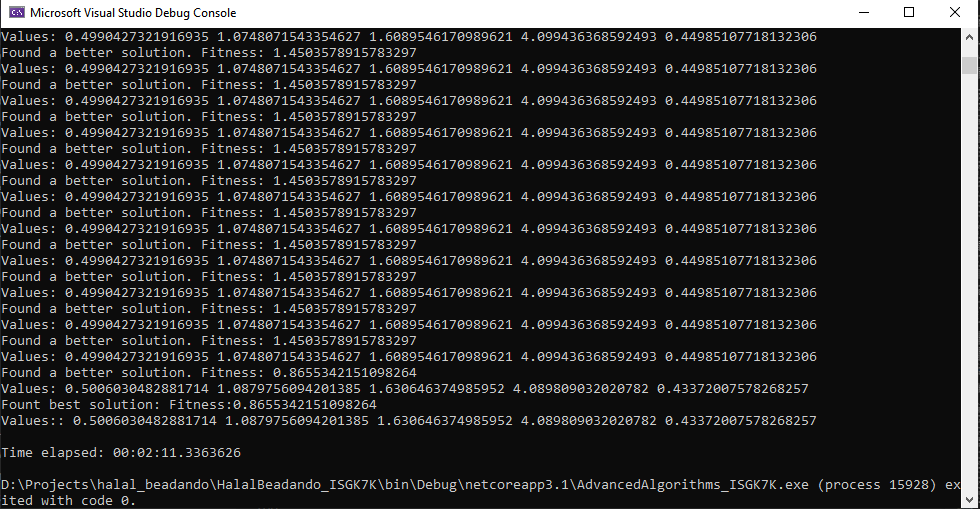
\includegraphics[width=1.0\textwidth]{genetic}

\section{Legkisebb körülíró poligon megoldása stochasztikus hegymászó algoritmussal}
\subsection{Bemenő paraméterek}

\begin{lstlisting}
  public class HCSettings
  {
        public int Epsilon;
        public int Dimension;
        public int MaxCoordinates;
        public double FitnessToReach;
        public string InputFilePath;
  }
\end{lstlisting}

\newpage
\subsection{Forráskód}
  \begin{lstlisting}
    public class SBPP_With_HC
    {
        static Random random = new Random();
        HCSettings settings;
        SmallestBoundaryPolygonProblem sBPP;

        public SBPP_With_HC(HCSettings settings)
        {
            this.settings = settings;
            sBPP = new SmallestBoundaryPolygonProblem(settings.InputFilePath);
        }

        public void SolveProblem()
        {
            Polygon polygon = InitalizePolygon();
            while (polygon.CalculateFitness(sBPP) > settings.FitnessToReach) // Stop condition
            {
                Polygon newPolygon = GenerateRandomPolygon(polygon);
                if(newPolygon.CalculateFitness(sBPP) < polygon.CalculateFitness(sBPP))
                {
                    polygon = newPolygon;
                    Console.WriteLine(String.Format("Found a better solution. Fitness: {0}, coordinates: {1}", polygon.CalculateFitness(sBPP), polygon.ToString()));
                }
            }
            Console.WriteLine(String.Format("Found best solution. Fitness: {0}, coordinates: {1}", polygon.CalculateFitness(sBPP), polygon.ToString()));
        }

        private Polygon InitalizePolygon()
        {
            Polygon polygon = new Polygon();
            for (int i = 0; i < settings.Dimension; i++)
            {
                polygon.Add(new Point() { x = random.Next(0, settings.MaxCoordinates), y = random.Next(0, settings.MaxCoordinates)});
            }
            return polygon;
        }

        private Polygon GenerateRandomPolygon(Polygon polygon)
        {
            Polygon newPolygon = new Polygon();
            foreach (Point point in polygon)
            {
                Point newPoint = new Point()
                {
                    x = point.x + random.Next(-1 * settings.Epsilon, settings.Epsilon),
                    y = point.y + random.Next(-1 * settings.Epsilon, settings.Epsilon)
            };
                newPolygon.Add(newPoint);
            }
            return newPolygon;
        }
    }
    \end{lstlisting}
  \subsection{Mérési eredmények}
  Megjegyzés: saját példámban a (200;200), (100;200), (200;100), (100;100) pontokat írtam körbe.
  \newline Beállított paraméterek:
  \begin{lstlisting}
    SBPP_With_HC sbppWithHc = new SBPP_With_HC(new HCSettings()
    {
      Epsilon = 10,
      Dimension = 3,
      MaxCoordinates = 400,
      FitnessToReach = 1.1,
      InputFilePath = "Input/Points.txt"
    });
  \end{lstlisting}
  Mérési eredmény:
  \begin{lstlisting}
    Found a better solution. Fitness: 131734.42199552144, coordinates:  (348,197)  (97,154)  (35,46)
    Found a better solution. Fitness: 129385.10352885423, coordinates:  (341,196)  (105,163)  (44,49)
    Found a better solution. Fitness: 124849.39250732775, coordinates:  (338,197)  (113,170)  (42,56)
    Found a better solution. Fitness: 123885.06863863926, coordinates:  (340,190)  (108,164)  (37,59)
    ...
    ...
    Found a better solution. Fitness: 1.1046079907893727, coordinates:  (383,199)  (158,73)  (-167,202)
    Found a better solution. Fitness: 1.1012255992045994, coordinates:  (378,201)  (164,75)  (-177,199)
    Found a better solution. Fitness: 1.100975070610763, coordinates:  (384,201)  (171,73)  (-183,199)
    Found a better solution. Fitness: 1.0955223765325635, coordinates:  (392,201)  (171,73)  (-191,199)
    Found best solution. Fitness: 1.0955223765325635, coordinates:  (392,201)  (171,73)  (-191,199)

    Time elapsed: 00:00:34.5222952
  \end{lstlisting}
  \subsection{Képernyőképek a futásról}
  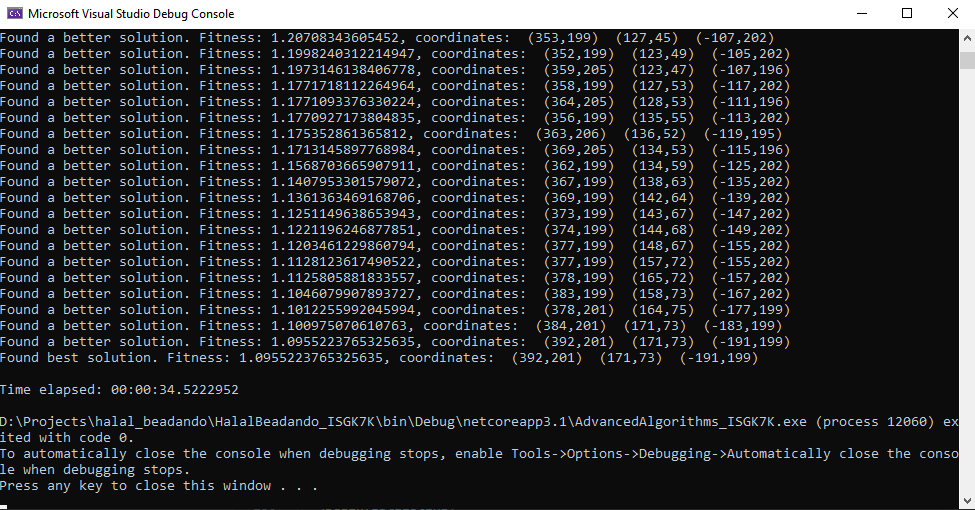
\includegraphics[width=1.0\textwidth]{hillclimbing}
  \section{Utazó ügynök probléma megoldása véletlen optimalizálással}
\subsection{Bemenő paraméterek}

\begin{lstlisting}
  public class ROSettings
  {
        public int Mean;
        public int Variance;
        public double FitnessToReach;
        public string InputFilePath;
  }
\end{lstlisting}

\subsection{Forráskód}
  \begin{lstlisting}
    public class TS_With_RO
    {
        Normal normal = new Normal();
        ROSettings settings;
        TravellingSalesmanProblem tSP;

        public TS_With_RO(ROSettings settings)
        {
            this.settings = settings;
            tSP = new TravellingSalesmanProblem(settings.InputFilePath);
        }

        public void SolveProblem()
        {
            Route route = tSP.BaseRoute;
            while (route.CalculateFitness(tSP) > settings.FitnessToReach) // Stop condition
            {
                Route newRoute = GenerateNewRoute(route);
                if (newRoute.CalculateFitness(tSP) < route.CalculateFitness(tSP))
                {
                    route = newRoute;
                    Console.WriteLine(String.Format("Found a better solution. Fitness: {0}", newRoute.CalculateFitness(tSP)));
                }

            }
            Console.WriteLine(String.Format("Found best solution. Fitness: {0}, coordinates:\n{1}", route.CalculateFitness(tSP), route.ToString()));
        }

        private Route GenerateNewRoute(Route route)
        {
            Route newRoute = Route.CreateCopy(route);
            MixRouteWithNormalDistribution(newRoute);
            return newRoute;
        }

        private void MixRouteWithNormalDistribution(Route route)
        {
            int n = route.Count;
            while (n > 1)
            {
                n--;
                int shift = (int)Normal.Sample(settings.Mean, settings.Variance);
                int randomIndex = n + shift;
                if (randomIndex < 0) randomIndex = 0;
                if (randomIndex >= route.Count) randomIndex = route.Count - 1;
                Town value = route[randomIndex];
                route[randomIndex] = route[n];
                route[n] = value;
            }
        }
    }
    \end{lstlisting}
  \subsection{Mérési eredmények}
  Beállított paraméterek:
  \begin{lstlisting}
    TS_With_RO tsWithRo = new TS_With_RO(new ROSettings()
    {
      FitnessToReach = 4500,
      Mean = 0,
      Variance = 2,
      InputFilePath = "Input/Towns.txt"
    });
  \end{lstlisting}
  Mérési eredmény:
  \begin{lstlisting}
    Found a better solution. Fitness: 8309.373046875
    Found a better solution. Fitness: 7920.33154296875
    Found a better solution. Fitness: 7882.4345703125
    Found a better solution. Fitness: 7816.77099609375
    Found a better solution. Fitness: 7773.91845703125
    Found a better solution. Fitness: 7444.97509765625
    Found a better solution. Fitness: 7437.162109375
    ...
    ...
    Found a better solution. Fitness: 4921.57763671875
    Found a better solution. Fitness: 4875.40576171875
    Found a better solution. Fitness: 4575.0498046875
    Found a better solution. Fitness: 4365.38916015625
    Found best solution. Fitness: 4365.38916015625, coordinates:
    (132,216)
    ...
    (150,224)

    Time elapsed: 00:02:06.0112957
  \end{lstlisting}
  \subsection{Képernyőképek a futásról}
  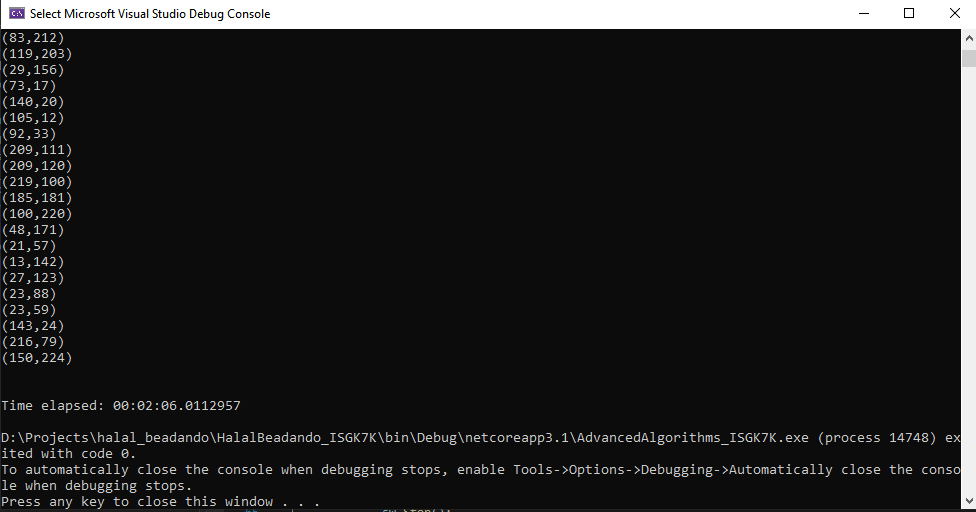
\includegraphics[width=1.0\textwidth]{random}
\end{document}